

\begin{table}[H]
    \centering
    \begin{tabular}{|c|c|c|c|}
    \hline
    \hline
        \textit{n} & $m=100g$ & $m=200g$ & $m=300g$ \\ 
        \hline
        \hline
        1 & 0.68 & 0.61 & 0.17 \\ 
        \hline
        2 & 0.60 & 0.70 & 0.27 \\ 
        \hline
        3 & 0.64 & 0.18 & 0.15 \\ 
        \hline
        4 & 0.63 & 0.11 & 0.10 \\ 
        \hline
        5 & 0.64 & 0.14 & 0.18 \\ 
        \hline
        \hline
    \end{tabular}
    \caption{Error Margin of the experimental data}
\end{table}

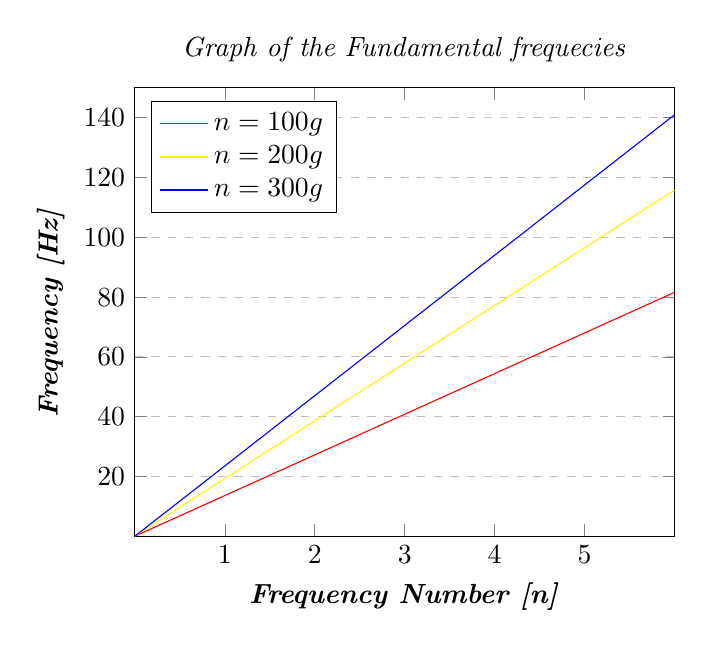
\begin{tikzpicture}
\begin{axis}[
                title={\textit{Graph of the Fundamental frequecies}},
                xlabel={\textbf{\textit{Frequency Number [n]}}},
                ylabel={\textbf{\textit{Frequency [Hz]}}},
                xmin=0, xmax=6,
                ymin=0, ymax=150,
                xtick={1,2,3,4,5},
                ytick={20,40,60,80,100,120,140},
                legend pos=north west,
                ymajorgrids=true,
                grid style=dashed,
                legend entries={$\frac{20\cdot\mu_0}{\pi}$ (\textit{Experimental})}
            ]
%Below the red parabola is defined
\addplot [
    domain=0:6, 
    samples=100, 
    color=red,
]
{13.6 * x};
\addlegendentry{$n = 100g$}

%Below the yellow parabola is defined
\addplot [
    domain=0:6, 
    samples=100, 
    color=yellow,
]
{19.3 * x};
\addlegendentry{$n = 200g$}

%Below the blue parabola is defined
\addplot [
    domain=0:6, 
    samples=100, 
    color=blue,
]
{23.5 * x};
\addlegendentry{$n = 300g$}

\end{axis}
\end{tikzpicture}

